\documentclass[12pt]{article}
\usepackage[unicode=true]{hyperref}
\usepackage[utf8x]{inputenc}
\usepackage{amsmath,amsthm,amsfonts,eucal}
\usepackage{graphicx}

\title{Applications of the Fresnel Integral}
\author{Jack Jones}
\date{March 17\th, 2019}


\newcommand\defbb[2]{\def#1{{\mathbb{#2}}}}
\newcommand\defbf[2]{\def#1{{\mathbf{#2}}}}
\newcommand\defcal[2]{\def#1{{\mathcal{#2}}}} % capital letters only
\newcommand\defrm[2]{\def#1{{\mathrm{#2}}}}
\newcommand\defsf[2]{\def#1{{\mathsf{#2}}}}
\newcommand\defvec[2]{\def#1{{\vec{#2}}}}
\def\vec{\mathbf}
\renewcommand\th[1][th]{$^{\text{#1}}$}

\let\C=\relax
\DeclareMathOperator\C{C} % C(x) := \int_0^x cos(t^2) \d{t}
\defbb\CC{C} % complex numbers
\defrm\ud{d}
\def\d#1{{\,\ud#1\,}}
\defrm\e{e}  % Euler's number
\DeclareMathOperator\erf{erf} % error function
\defsf\si{i} % \sqrt{-1}
\defbb\R{R}
\let\S=\relax
\DeclareMathOperator\S{S} % S(x) :=int_0^x sin(t^2) \d{t}


\begin{document}
\maketitle
\begin{abstract}
	
\end{abstract}
\clearpage


\section{Introduction}

\subsection{Definition of the Fresnel Integral}
The Fresnel integrals are two transcendental functions defined as follows
\begin{align}
  \S(x) &:= \int_0^x  \sin(\frac\pi2 t^2) \d{t}, \\
  \C(x) &:= \int_0^x \cos(\frac\pi2 t^2) \d{t}.
\end{align}
The difficulty is that these integrals cannot be computed with analytic means, i.e.~the functions are transcendenta \cite[p.195ff]{AS}.  This is in contrast to, e.g.
$$ \int_0^x (\sin t)^2 \d{t} = \frac12\int_0^x \left(1-\cos(2t)\right)\d{t} = \frac12x -\frac14\sin(2x).
$$

\subsection{Some simple history}
The Fresnel integral and the related Euler spiral were discovered multiple times during history.  One of the first occurrances is according to \cite{Lev08} by J. Bernoulli in 1694 where he defines a curve such that an ideal metal rod of this shape unwinds to a straight line when placed under load at the ends.  In 1744 Euler is able to describe the curve by a differential equation that also allows him to reformulate it as the Fresnel integral.  37 years later he is able to compute the limiting points ($t\to\pm\infty$) of the curve and integrals.  Fresnel rediscovers the curve in 1818 and successfully applies it to the diffraction on a slit \cite{Lev08}.  He is also able to compute a couple of values numerically.  In 1874 Cornu plotted the curve accurately and proposes it as a graphical means for computing diffraction problems.


\section{Properties}
\subsection{Basic properties}
The Fresnel integrals are odd, i.e.
\begin{align*}
	\S(-x) &= \S(x), & \C(-x) &= \C(x).
\end{align*}
\begin{proof}[Idea of proof]  The integrands $\sin(t^2)$ and $\cos(t^2)$ are even in $t$ and an anti-derivative $F(x)$ of an even function is odd if in addition $F(0)=0$.  The latter follows, because both integrals start at $t=0$.
\end{proof}

Their limits are
\[  \lim_{x\to\infty} \S(x) = 0.5\sqrt{\tfrac\pi2},\qquad  \lim_{x\to\infty} \C(x) = 0.5\sqrt{\tfrac\pi2}.
\]

Since the integrals cannot be computed by elementary analytic means, an alternative is to compute them with a power series.  Therefore we present the Taylor expansion as
\begin{align*}
  \S(x) &= \sqrt{\frac\pi2}\sum_{n\ge0} (-1)^nx^{4n+3}\frac{(\pi/2)^{2n+1}}{(2n+1)!(4n+3)}, \\
  \C(x) &= \sqrt{\frac\pi2}\sum_{n\ge0} (-1)^nx^{4n+1}\frac{(\pi/2)^{2n}}{(2n)!(4n+1)}.
\end{align*}
\begin{proof}[Idea of proof]  Start from the well known Taylor expansion of $\sin t = \sum_{n\ge0}$ $(-1)^n t^{2n+1}/(2n+1)!$ and $\cos t = \sum_{n\ge0} (-1)^nt^{2n}/(2n)!$, substitute $t\mapsto \tfrac\pi2 t^2$ and take the antiderivative for each summand.  The resulting series are $\S(t)$ and $\C(t)$, because the integral of an absolutely converging power series equals the absolutely converging power series of the integrals of the summands.
\end{proof}

\begin{figure}[h!]
	\centering
	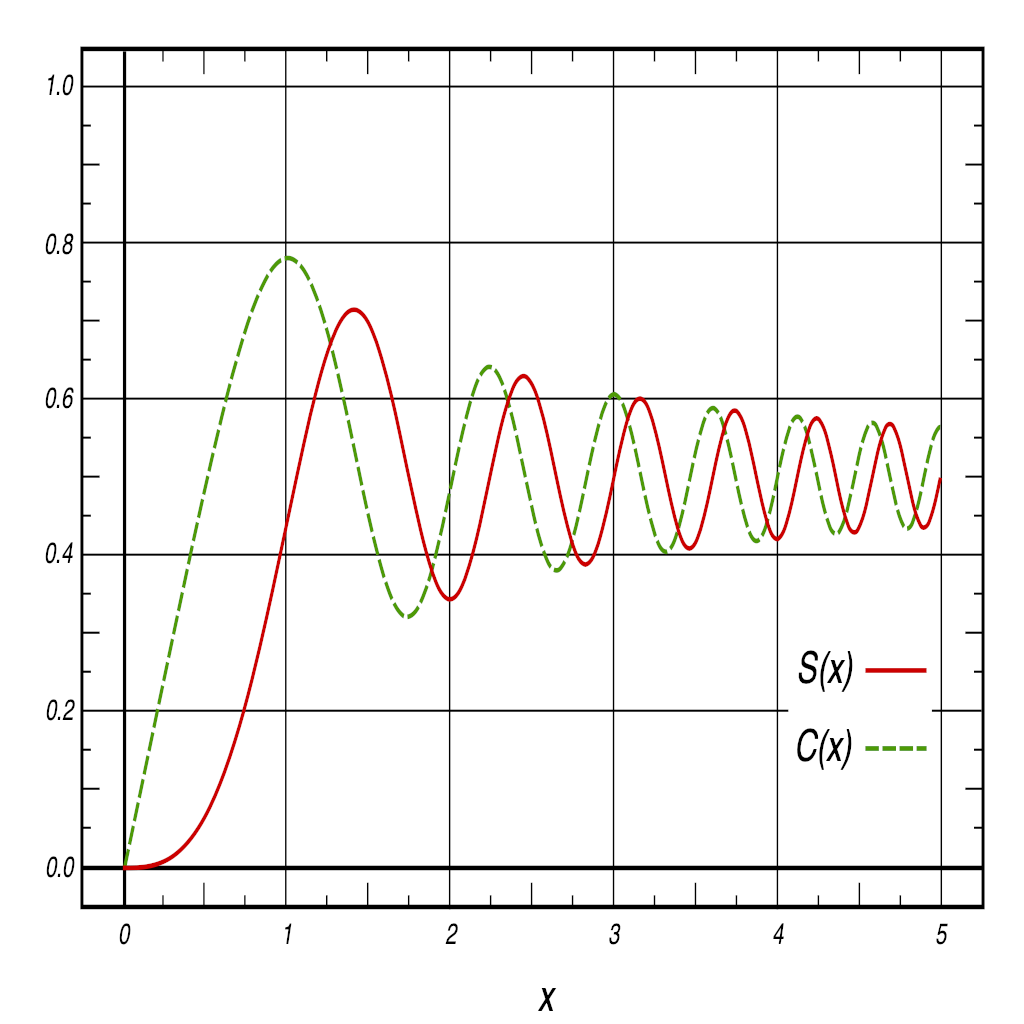
\includegraphics[width=0.5\textwidth]{Fresnel-Integrals-(Normalised).png}
	\caption{Fresnel integrals.  Taken from \cite[/Fresnel\_Integral]{wiki}.}
\end{figure}


\subsection{Other expressions}
The Fresnel integrals are closely related to the error function which is defined as follows
$$  \erf(x) := \int_{-x}^x \exp(-t^2) \d{t}.
$$
Also this function is analytic and can therefore be expanded to the whole complex plane.  Here the integral for fixed endpoints is independent of the path.

Now for the complex defintion of exponential function
\begin{align*}  \exp(x+\si y) &:= (\cos y +\si\sin y)\e^x
\intertext{we obtain}
  \C(z)+\si\S(z) &= \int_0^z \exp\left(\si\frac\pi2 t^2\right)\d{t} 
\intertext{Now we do a substitution in the complex plane as $t'=\sqrt{i}t$, i.e.~$\d{t'}=\frac{1+\si}{\sqrt{2}}\d{t}$ and obtain}
  &= \frac{1-\si}{\sqrt{2}}\int_0^{\frac{1+\si}{\sqrt{2}}} \exp(t^{\prime2}) \d{t'} = \frac12\,\frac{1-\si}{\sqrt2} \erf\left(\frac{1+\si}{\sqrt2}\,\frac\pi2 z\right).
\end{align*}
Therefore we can say that the Fresnel integrals are the real and imaginary part of the complex error function.

\section{Euler Spiral}
\cite{Lev08}  The Euler spiral is a curve in the complex plane that has curvature proportional to the arc length.  Here arc length is defined as
\[  s(T) := \int_0^T \sqrt{\d{x}^2+\d{y}^2}
\]  for some differentiable curve $(x(t),y(t))$ in the plane.  Note that the curve length is monotone increasing with the parameter $t$ of the curve.  For a nice curve, it is possible to reparametrize the cruve in the arc length, i.e.~$(x(s),y(s))$.

The curvature of a smooth curve is defined as 
\[  \kappa=\frac1R = \frac{\dot x\ddot y -\ddot x\dot y}{(\dot x)^2+(\dot y)^2}.
\]  Here $\dot{x}=\frac{\d{x}}{\d{t}}$ is the derivative by the parameter $t$ (and $\dot{y}$ that of $y(t)$ and $\ddot{x}$ the second derivative, correspondingly).  If we combine the coordinates to a complex number $z=x(t)+\si y(t)$ and reparametrize the curve in its arc length $z(s)$, then the curvature condition reads as
\[  z^{\prime\prime}\bar{z}' = \frac\si{R} = \si s.
\]  Here $z'=\frac{\d{z}}{\d{s}}$ is the derivative by the arc length.

\begin{itemize}\item The definition of Euler Spiral
\item The relation between Fresnel Integral and Euler Spiral
\end{itemize}


\section{Application of Fresnel Integral}
\subsection{Application using the Euler Spiral}
\cite{BH12}
Electromagnetic field intensity

\subsection{Further Applications}


\section{Conclusion}

\bibliographystyle{alphasorteprint}
\bibliography{bibliography.bib}
\nocite{AS, BE, Sim, Str, WW}  % TODO: place in text
\end{document}
